\documentclass{article}
\usepackage[utf8]{inputenc}
\usepackage{geometry}
\usepackage{graphicx}
\usepackage{pgfplots}
\usepackage{verbatim}
\usepackage{amssymb}
\usepackage{amsmath}

\geometry{a4paper, left=2cm, right=2cm, top=1cm, bottom=2cm}

\begin{document}

\begin{minipage}{0.7\textwidth}
    \small \textbf{MECÁNICA VECTORIAL}  \\
    \small {Facultad de Ciencias, Universidad Nacional Autónoma de México} \\
    \small {Fecha de entrega: 01 de Marzo de 2023} \\
    \small {Nombre completo: Andrés López González} \\
    \small {Tarea número 4}
\end{minipage}
\hfill
\begin{minipage}{0.12\textwidth}
    
\includegraphics[width=\linewidth]{logo_universidad}
\end{minipage}

\section{Preguntas.}
XVIII. Usted arroja una pelota desde un acantilado a una velocidad inicial de 15 m/s y con un ángulo de 20° abajo de la horizontal. Halle (a) su desplazamiento horizontal, y (b) su desplazamiento vertical 2.3 s más tarde.\\\\

\textit{Por la componente en x tenemos el siguiente desplazamiento no acelerado definido por.}
\begin{align*}
    x_0(t) &= v_{0x}t + \frac{at^2}{2} \\
    &= v_0t \\
    &= |v_0|\cos(\phi)t \\
    &= 15\cos(\phi)t \\
    &= 15\cos(20)t \\
\end{align*}
\textit{Por la componente en y tenemos un análisis similar, sin embargo, aquí la velocidad inicial es cero y la aceleración es la gravitacional.}
\begin{align*}
    y_0(t) &= v_{0y}t - \frac{gt^2}{2} \\
    &= 15\sin(-20)t - \frac{9.806t^2}{2} \\
\end{align*}
\textit{Entonces obtenemos la siguiente función de posición respecto al tiempo, y evaluamos en el tiempo solicitado}
\begin{align*}
    \Vec{r}(t) &= (15\cos(\phi)t,- \frac{9.806t^2}{2})
\end{align*}
\textit{Evaluando en $t=2.3$}
\begin{align*}
    \Vec{r}(t) &= (15cos(20)\cdot(2.3s), 15\sin(-20)\cdot(2.3s) - \frac{9.806\cdot(2.3s)^2}{2} \\
    &= (32.41939, -37.73656)
\end{align*}\\\\
\textit{Su desplazamiento horizontal y vertical en el tiempo indicado es $(x,y) = (32.41939, -37.73656)$.}

XXVII. Un malabarista maneja cinco bolas en movimiento, lanzando cada una secuencialmente hacia arriba a una distancia de 3.0 m. (a) Determine el intervalo de tiempo entre dos lanzamientos sucesivos. (b) De las posiciones de las otras bolas en el instante en que una llega a su mano. (Desprecie el tiempo tomado para transferir la bola de una
mano a la otra.)\\
\textit{Determinaré cuánto es la velocidad vertical inicial.}
\begin{align*}
    \Delta y_f &= -3m = v_0yt - \frac{gt^2}{2} \\
    &= - \frac{gt^2}{2} \\
    \Rightarrow t^2 &= \frac{-2\Delta y_f}{g} \\
    &= \frac{-2 \cdot -3}{9.806}m \\
    \Rightarrow t &= \sqrt{\frac{6}{9.806}} \\
    &\approx 0.782222s \\
    \Rightarrow t_{Total} &= 2\cdot 0.782222s \approx 1.564444s
\end{align*}

\begin{figure} [h]
    \centering
    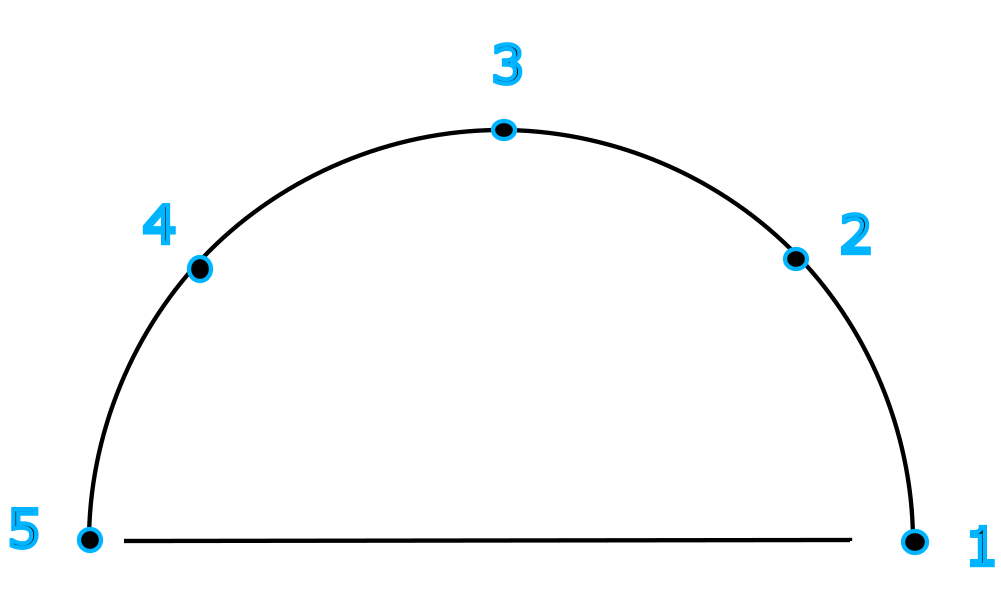
\includegraphics[width=0.5\linewidth]{Malab.png}
    \caption{Descripción del fenómeno}
    \label{fig:enter-label}
\end{figure}
\textit{Si tarda 1.564444s en un recorrido al cual le siguen las otras 4 pelotas entonces cada pelota tardará un quinto de ello, es decir, \textbf{el intervalo entre lanzamientos es 0.312888s}.}\\\\
\textit{Las posiciones de cada bola en el instante que una llega si consideramos el dibujo que he trazado son simétricas la primera y la última de modo que $y_5=y_1=0$ y $y_3=3$, considerar la segunda y cuarta bola en la misma posición es un error pues si recordamos el problema del basquetbolista en la cresta suelen ocurrir situaciones contraintuitivas. Calculemos en qué posición está $y_2$ y $y_4$, recordemos que nuestro sistema de referencia tiene el origen fijado en la base.}
\[ \Delta y_2 = v_0t - \frac{gt^2}{2} = v_0(0.312888) - \frac{9.806(0.312888)^2}{2} \]
\textit{Para la velocidad inicial tomamos la velocidad final como cero pues es cuando llega a su punto más alto, ya conocemos cuanto tarda en llegar a ese punto entonces es fácilmente despejable.}
\[ 0 = v_0 - gt \quad \Rightarrow \quad v_0 = gt = 9.806 \cdot 0.782222 \approx 7.670468932 \frac{m}{s} \]
\textit{Retomamos nuestra posición en y.}
\[ \Delta y \approx (7.670468932)(0.312888) - \frac{9.806(0.312888)^2}{2} \approx 1.91999m \]
\textit{Análogamente con $\Delta y_4$}
\[ \Delta y_2 = v_0t - \frac{gt^2}{2} = (7.670468932)(3\cdot0.312888) - \frac{9.806(3\cdot0.312888)^2}{2} \approx 2.88000m \]
\textit{Con esto ya tenemos las tres posiciones del ejercicio.}\\\\

XXXV. A qué velocidad inicial deberá el jugador de baloncesto lanzar la pelota, formando 55° con la horizontal, para encestar el tiro de castigo, como se muestra en la figura 30? El aro de la cesta tiene un diámetro de 18 in. Obtenga otros datos de la figura 30. \\
\begin{figure} [h]
    \centering
    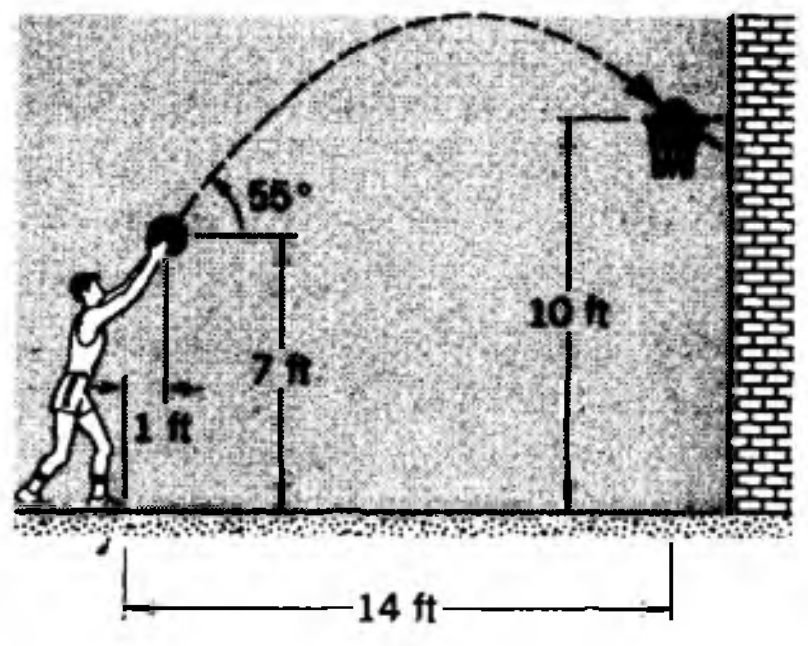
\includegraphics[width=0.25\linewidth]{F30.png}
    \caption{Imagen descriptiva.}
\end{figure}\\
\textit{Ocuparemos la fórmula de la norma de la velocidad tangencial cero en un tiro parabólico, recordamos que el ángulo inicial es de 55 grados, el delta x es 13 pies pues se le sustrajo uno entre el brazo y la persona, la gravedad en sistema inglés es 32.3$\frac{ft}{s^2}$, finalmente el desplazamiento en y será la altura de la canasta menos la altura entre el suelo y el balón $(10-7)ft=3ft$. Ahora sí aplicamos en este problema de recetario de cocina.}
\begin{align*}
    v_o &= \sqrt{\frac{\Delta x^2g}{2\cos^2(\vartheta)(\Delta x \tan(\vartheta) - \Delta y)}} \\
    &= \sqrt{\frac{169ft^2\cdot32.2\frac{ft}{s^2}}{2\cos^2(55^{\circ})(13ft \tan(55^{\circ}) - 3ft)}} \\
    &= 23.05035 \frac{ft}{s^2}
\end{align*}





LIII. Un satélite de la Tierra se mueve en una órbita circular situada a 640 km sobre la superficie de la Tierra. El tiempo para una revolución es de 98.0 min. (a) ¿Cuál es
la velocidad del satélite? (b) ¿Cuál es la aceleración en caída libre en la órbita? \\

\textit{Para calcular la velocidad del satélite convertiremos el período de 98.0 minutos a un factor más intuitivo que es segundos multiplicándolo por 60.} \\
\[ 98min \cdot \frac{60s}{1min} = 5,880s \]
\textit{Ahora, podemos utilizar la fórmula de la circunferencia para hallar la distancia recorrida por el satélite durante una órbita asumiéndola completamente redonda (si fuera geoide ni en maestría puedo resolverlo xd). Y ese resultado lo dividimos entre el tiempo para obtener la velocidad en $\frac{km}{s}$. Recordemos que el radio de la Tierra según los datos del Resnick es 6,378km} \\
\[ v = \frac{d}{t} = \frac{2 \pi r}{t} \approx \frac{2\cdot 3.14159265358979 \cdot (6,378 + 640km)}{5,880s} \approx 7.49921 \frac{m}{s} \]
\textit{Ahora calculemos la aceleración en caída libre en la órbita, con esto entendemos que es la aceleración que te atrae como usualmente lo hace la gravedad, i.e. hacia el centro de la tierra, lo que coincide con la aceleración centrípeta.}
\[ a_{centripeta} = \frac{v^2}{r} \approx \dfrac{7.49921^2}{6,378 + 640}\frac{km}{s} \cdot \frac{1,000m}{km} \approx 8.01341 \frac{m}{s^2} \]


\end{document}